\documentclass[aps,showpacs,twocolumn,floats,prd,superscriptaddress,nofootinbib]{revtex4-1} 
\usepackage{graphicx,amsmath,amssymb,amstext}
\usepackage{amssymb,amsbsy,amsfonts,amsthm,color}

\usepackage{epsfig}
%\usepackage{showkeys}
\usepackage{graphicx}
\usepackage{subfigure}

\graphicspath{{Figures/}}

\begin{document}

\title{Pulsar Acceleration Shifts from nearby Supernova Explosion}

\author{Darsh Kodwani}
\email{dkodwani@physics.utoronto.ca}
\affiliation{Canadian Institute of Theoretical Astrophysics, 60 St George St, Toronto, ON M5S 3H8, Canada.}
\affiliation{University of Toronto, Department of Physics, 60 St George St, Toronto, ON M5S 3H8, Canada.}

\author{Ue-Li Pen}
\email{pen@cita.utoronto.ca}
\affiliation{Canadian Institute of Theoretical Astrophysics, 60 St George St, Toronto, ON M5S 3H8, Canada.}
\affiliation{Canadian Institute for Advanced Research, CIFAR program in Gravitation and Cosmology.}

\author{I-Sheng Yang}
\email{isheng.yang@gmail.com}
\affiliation{Canadian Institute of Theoretical Astrophysics, 60 St George St, Toronto, ON M5S 3H8, Canada.}
\affiliation{Perimeter Institute of Theoretical Physics, 31 Caroline Street North, Waterloo, ON N2L 2Y5, Canada.}

\begin{abstract}
We show that when a supernova explodes, a nearby pulsar goes through two changes in the time-derivative of its period. A stable, millisecond pulsar can allow us to measure such effect. This may improve our measurement on the total energy released in neutrinos and also the actual orientation of the supernova-pulsar system. A joint timing of a few pulsars can even triangulate the location of a hidden supernova.
\end{abstract}

\maketitle

\section{Introduction and Summary}

When a supernova (SN) explodes, it releases a fraction of solar-masses energy in shell of relativistic neutrinos. Although neutrinos barely interact with other matter directly, relocating such amount of mass inevitably affects the background geometry. If an accurate timing apparatus is nearby, such as a millisecond pulsar, then one can hope to observe a measurable effect. The purpose of this paper is to calculate such effect and provide a better idea of how useful such an observation can be.

Since this neutrino shell is very thin---passing through either the Earth or the pulsar in a time much shorter than the typical duration for timing observations---we can treat it as a co-dimension-1 delta-function and describe the spacetime by Israel Junction Conditions (IJC) \cite{Isr66}. Furthermore, we will treat both the neutrinos and the pulsar signal as propagating at the speed of light. In reality that is not exactly true, with photons moving even slower than neutrinos. Nevertheless, the time delay is again much shorter compared to the duration of timing observations, thus it does not invalidate our result. The analytical model then becomes extremely simple, since it involves nothing but tracking geodesics\cite{BouFre07,JohYan10}.

In Sec.\ref{sec-JC}, we present the general setup of geometry with junctions. In Sec.\ref{sec-1+1} we study the scenario in which the SN and the pulsar are exactly aligned, as shown in Fig.\ref{fig:1}. On one hand, this is the simplest scenario as it reduces to a (1+1) dimensional problem. On the other hand, this might have the strongest observable effect. After all, the signals that arrive right before and right after the neutrino shell travelled in two dramatically different geometries. We show that there is no sudden change in the pulse period.
% More precisely, the observed pulsar period cannot jump across the neutrino shell. In hindsight, these should not be too surprising, as they follow from the physical continuation of spacetime. Although the metrics on either side of the neutrino shell looks very different, the physical distance between two points, and the relative velocity between two points, cannot change discontinuously. The first fact follows directly from the first of IJC, while the second fact requires the notion of continuing a geodesic across a junction , for which we will provide more explicit details.
The leading observable effect is in its derivative, due to the change in gravitational acceleration felt by the pulsar. 
\begin{equation}
\Delta(\dot{P}/P) \sim -\Delta M / r_p^2~,
\label{eq-main}
\end{equation}
where $P$ is the spin period, $G$ and $c$ are set to 1, $\Delta M$ is the total neutrino shell mass thus also its effective Schwarzschild radius, and $r_p$ is the distance between the SN and the pulsar. 

In Sec.\ref{sec-3d}, we study the general case in which the pulsar and SN are not aligned. We demonstrate that the acceleration changes twice. First when we observe the SN explosion, and the second time when the neutrino shell reaches the pulsar. Both changes have roughly the same amplitude as Eq.~(\ref{eq-main}), but can have different signs due to the actual SN-pulsar orientation. 

In Sec.\ref{sec-obs}, we show that the required timing accuracy to measure such acceleration change is the light-crossing time of the effective Schwarzschild radius of the neutrino shell. That is about $10^{-6}$ seconds, which is achievable by millisecond pulsars. The values of these two changes may allow us to better determine the total energy released in neutrinos and the actual orientation of the SN-pulsar system.

\section{Geometry}
\label{sec-JC}

We will calculate the observable effect by treating the spacetime around the SN as roughly a Schwarzschild geometry, while the pulsar is like a test particle in this background.
\begin{equation}
	ds_i^2 = -\left( 1 -\frac{2M_i}{r}\right) dt_i^2 + \left( 1 -\frac{2M_i}{r} \right)^{-1} dr^2 + r^2 d \Omega_2^2~.	\label{2.1}
\end{equation}
Here the $i$ index on quantities stands for the ``initial" spacetime, thus $M_i$ is the total mass of the SN (before it loses the neutrino shell). Similarly, replacing $i$ by $f$ means the final spacetime where $\Delta M = (M_i-M_f)$ is the total energy carried away by the neutrino shell. In principle every coordinate should have a subscript $i$ or $f$. However, since we assume spherical symmetry, we can identify their angular coordinates and declare the radial coordinate as the area radius of the two-sphere. Thus, the only coordinate difference appears in $t_i$ and $t_f$. 

The initial and final geometries are connected through a junction, which is the neutrino flow that we treat as a thin, null shell. The radial 4-vector of this shell is thus a null vector, which can be represented in either coordinate.
\begin{eqnarray}
j_\mu &\equiv& \left( \left(1-\frac{2M_i}{r}\right)^{-1} ,  1 , 0 , 0 \right)_{\rm in \ metric \ i}~.
\end{eqnarray}
Throughout this paper, we will use ``$\equiv$'' for how to represent a physical quantity in a coordinate system. In the ``final" metric, one replaces the ``$i$'' in the above expression by ``$f$''. That leads to a mathematically different component form, but it represents the same physical 4-vectors.

We will treat our signal as photons and talk about the change of frequencies. In reality, one just relates this to the pulsar period by $w=(2\pi/P)$. A photon can be described by a null-4-vector with a fixed normalization as shown in section 25.6 of \cite{MTW}. In a fixed Schwarzschild geometry, the general form is
\begin{equation}
	k^\mu \equiv w_{\infty}\left( \frac{1}{(1- \frac{2M}{r})}, \sqrt{ 1 - \frac{b^2}{r^2} \left( 1 - \frac{2M}{r} \right)}, \frac{b}{r^2}, 0 \right)~. \label{eq-photon}	
\end{equation}
The overall normalization $w_{\infty}$ is defined as the frequency observed by an asymptotic observer at rest, and the fixed angular momentum is parametrized by the impact parameter $b$. For convenience, we can always assume that the motion is confined to the equator of the two sphere.

\section{The Aligned Case}
\label{sec-1+1}

Now we will consider the case that $b=0$ in Eq.~(\ref{eq-photon}), namely the SN, the pulsar, and the earth sit on one straight line, and the pulsar is in the middle. This reduces to a (1+1)-dimensional problem as depicted in Fig.\ref{fig:1}. In this scenario, the earth will receive two photons from the SN, one right after the other, but they have traveled through two distinctly different geometries. One might suspect a sudden and dramatic change in the signal, but it is easy to show otherwise.

\begin{figure}[tb!]
\begin{center}
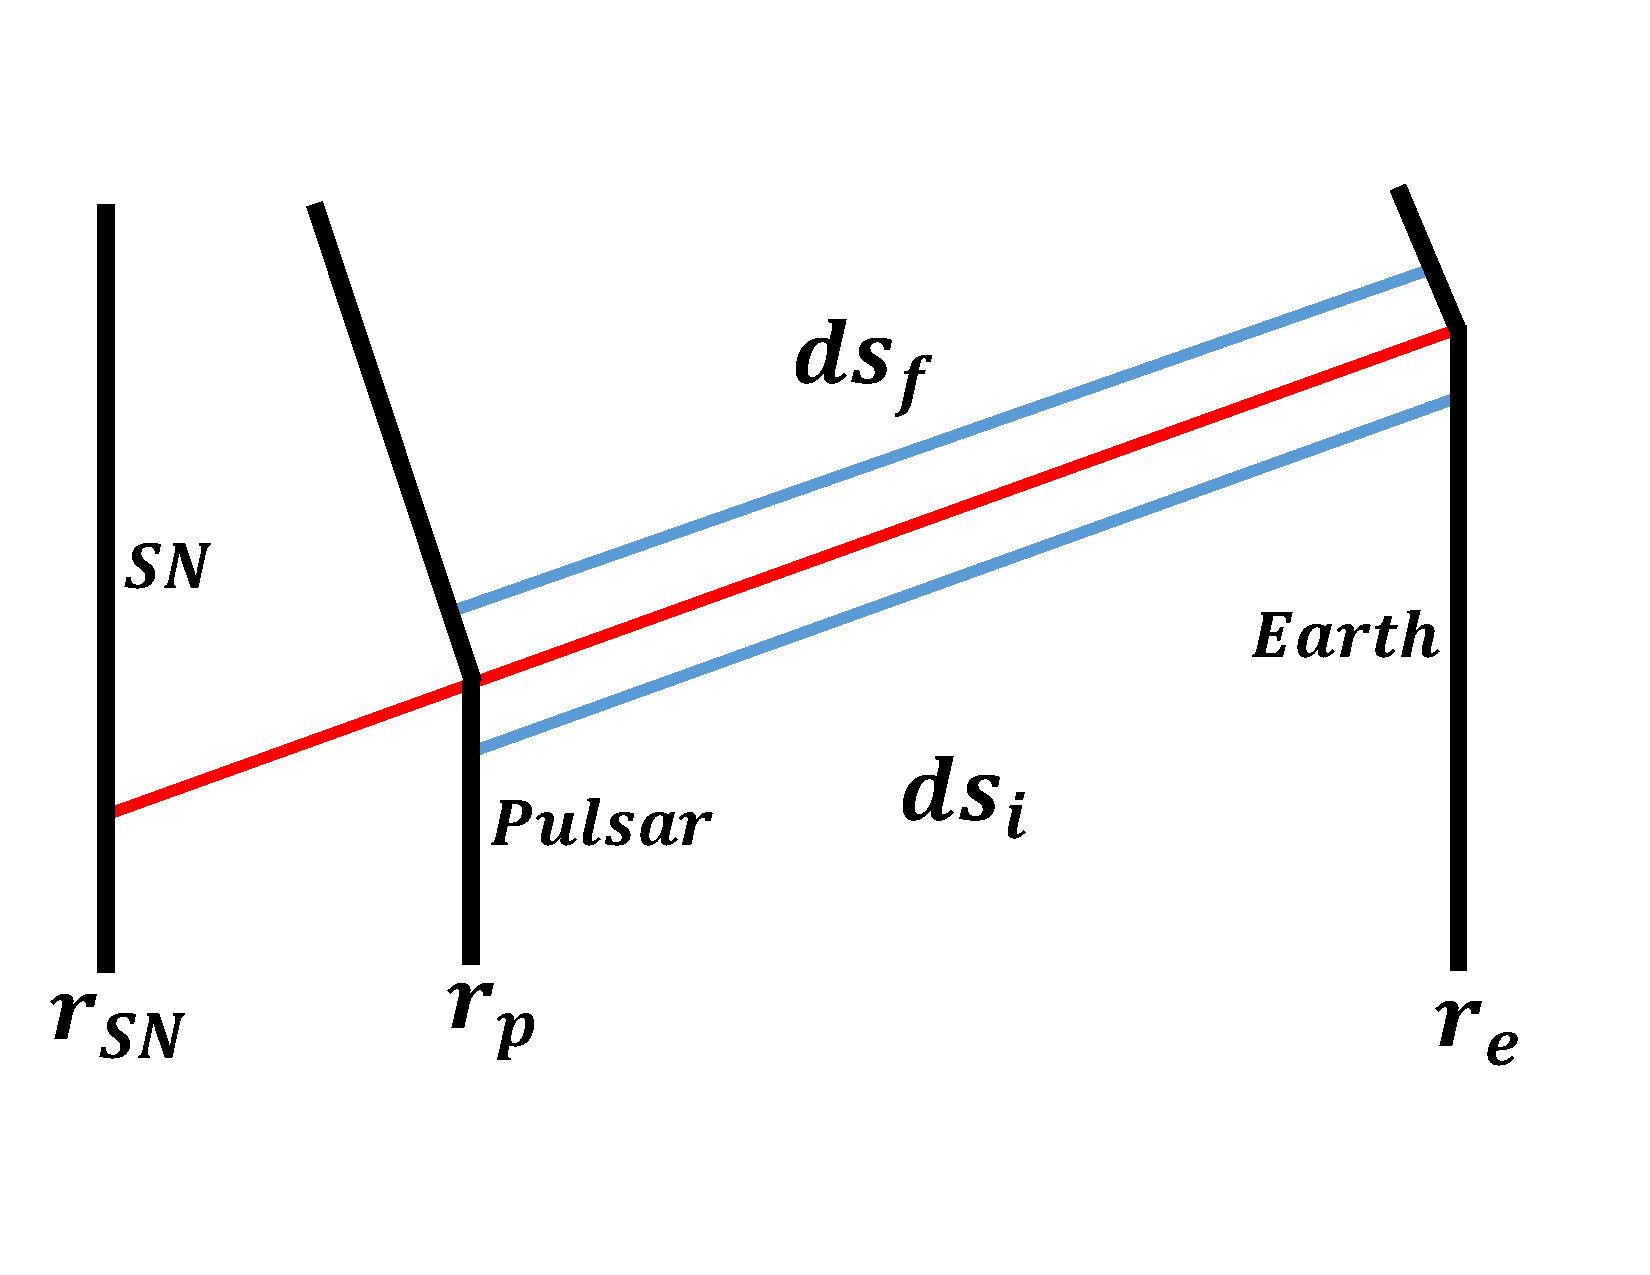
\includegraphics[scale = 0.3]{Image2.pdf}
\caption{Spacetime diagram showing the position of the pulsar, $r_p$, earth, $r_e$, and the SN, $r_s$. The red line represents the neutrino null vector and the blue lines represent the photon trajectories.}
\label{fig:1}
\end{center}
\end{figure}

Let $p_\mu$ and $e_\mu$ be the timelike 4-vectors of the pulsar and the earth while emitting/receiving these pair of photons. Continuity across the junction implies the following constraint on how they are represented in either geometry.
\begin{eqnarray}
p_\mu j^\mu(r_p)_{\rm \ in \ metric \ i} &=& 
p_\mu j^\mu(r_p)_{\rm \ in \ metric \ f}~,
\label{eq-JuncPuls} \\ 
e_\mu j^\mu(r_e)_{\rm \ in \ metric \ i} &=& 
e_\mu j^\mu(r_e)_{\rm \ in \ metric \ f}~.
\end{eqnarray}
The two photons are defined by the physical fact that in the rest frame of the pulsar, they have the same frequency.
\begin{equation}
w_p = -p_\mu k^\mu(w^i_\infty, r_p)_{\rm i} = 
-p_\mu k^\mu(w^f_\infty, r_p)_{\rm f}~.
\label{eq-PulsEmit}
\end{equation}
It is then straightforward to combine these 3 equations to show that the frequencies received on earth are identical.
\begin{equation}
w_e = -e_\mu k^\mu(w^i_\infty, r_p)_{\rm i} = 
-e_\mu k^\mu(w^f_\infty, r_p)_{\rm f}~.
\end{equation}

\subsection{Leading order expansion and physical intuition}

Our conclusion above is exactly correct in full nonlinear general relativity, although it might be surprising to some readers. Here we will expand the two steps separately to leading order for better physical intuitions. First of all, it is quite realistic to set $r_e \gg r_p$ and treat it as being infinite, so the only physical change happens in the pulsar.

Instead of using Eq.~(\ref{eq-JuncPuls}), if we had assumed that the pulsar is at rest in both geometries before and after the neutrino shell crosses, then we would have derived a frequency ratio of $[1-\Delta M/r_p]$ between these two photons\footnote{In fact, any non-relativistic initial velocity leads to this result.}. This would have reflected the fact that they climbed out of two different gravitational potentials, but it cannot be the full story. If the pulsar was at rest before the neutrino shell hits it, Eq.~(\ref{eq-JuncPuls}) demands that it picks up a velocity in the new coordinate
 \begin{eqnarray}
p_\mu &\equiv& \left( \left( 1 - \frac{2M_i}{r} \right)^{-\frac{1}{2}}, 0, 0,0\right)_{\rm i} 
\label{eq-PulsarRest} \\ \nonumber  &\equiv&	
\left( \left( 1 - \frac{2M_f}{r} \right)^{-\frac{1}{2}}, -\frac{\Delta M}{r_p},0,0 \right)_{\rm f}~.
\end{eqnarray}
The new velocity, $v=\Delta M/r_p$, is falling toward the SN remnant. This then creates a Doppler shift that exactly cancels the difference in gravitational potential, thus netting no frequency change.\footnote{This change in coordinate velocity is not due to any direct interaction with the neutrino shell, but simply an artifact of coordinate change across the junction.}
\begin{equation}
(w_e)_{\rm i} \equiv w_p \left(1-\frac{M_i}{r_p}\right) = 
w_p (1-v)\left(1-\frac{M_f}{r_p}\right) \equiv (w_e)_{\rm f}~.
\label{eq-leading}
\end{equation}

\subsection{Observable change in acceleration}
\label{sec-acceleration}

Let us continue the approximation in the previous section and take a time derivative on Eq.~(\ref{eq-leading}). Realistically, $v \ll1$ and $r_p\gg M$, then the dominant change in time comes from the velocity.
\begin{equation}
\frac{\dot{w_e}}{w_e} = -\dot{v} = -\frac{M}{r_p^2}~.
\label{eq-AccChange}
\end{equation}
When the pulsar crosses the neutrino shell, the enclosed mass certainly changes from $M_i$ to $M_f$, and $\dot{w_e}$ indeed changes suddenly. It is not a suddenly observable change, since the change in $w_e$ needs some time to build up before it is observable. Nevertheless, this is the leading order observable for us.

\section{General Cases}
\label{sec-3d}

In general, the three bodies in this problem will not exactly align. Let $\theta$ be the angle between $r_p$ and $r_e$ as shown in Fig.\ref{fig:3}, we will calculate the general change in acceleration in the same assumption that has a convenient 1st order expansion: $r_e\gg r_p\gg M$ and a non-relativistic initial velocity.

\begin{figure}[t]
\begin{center}
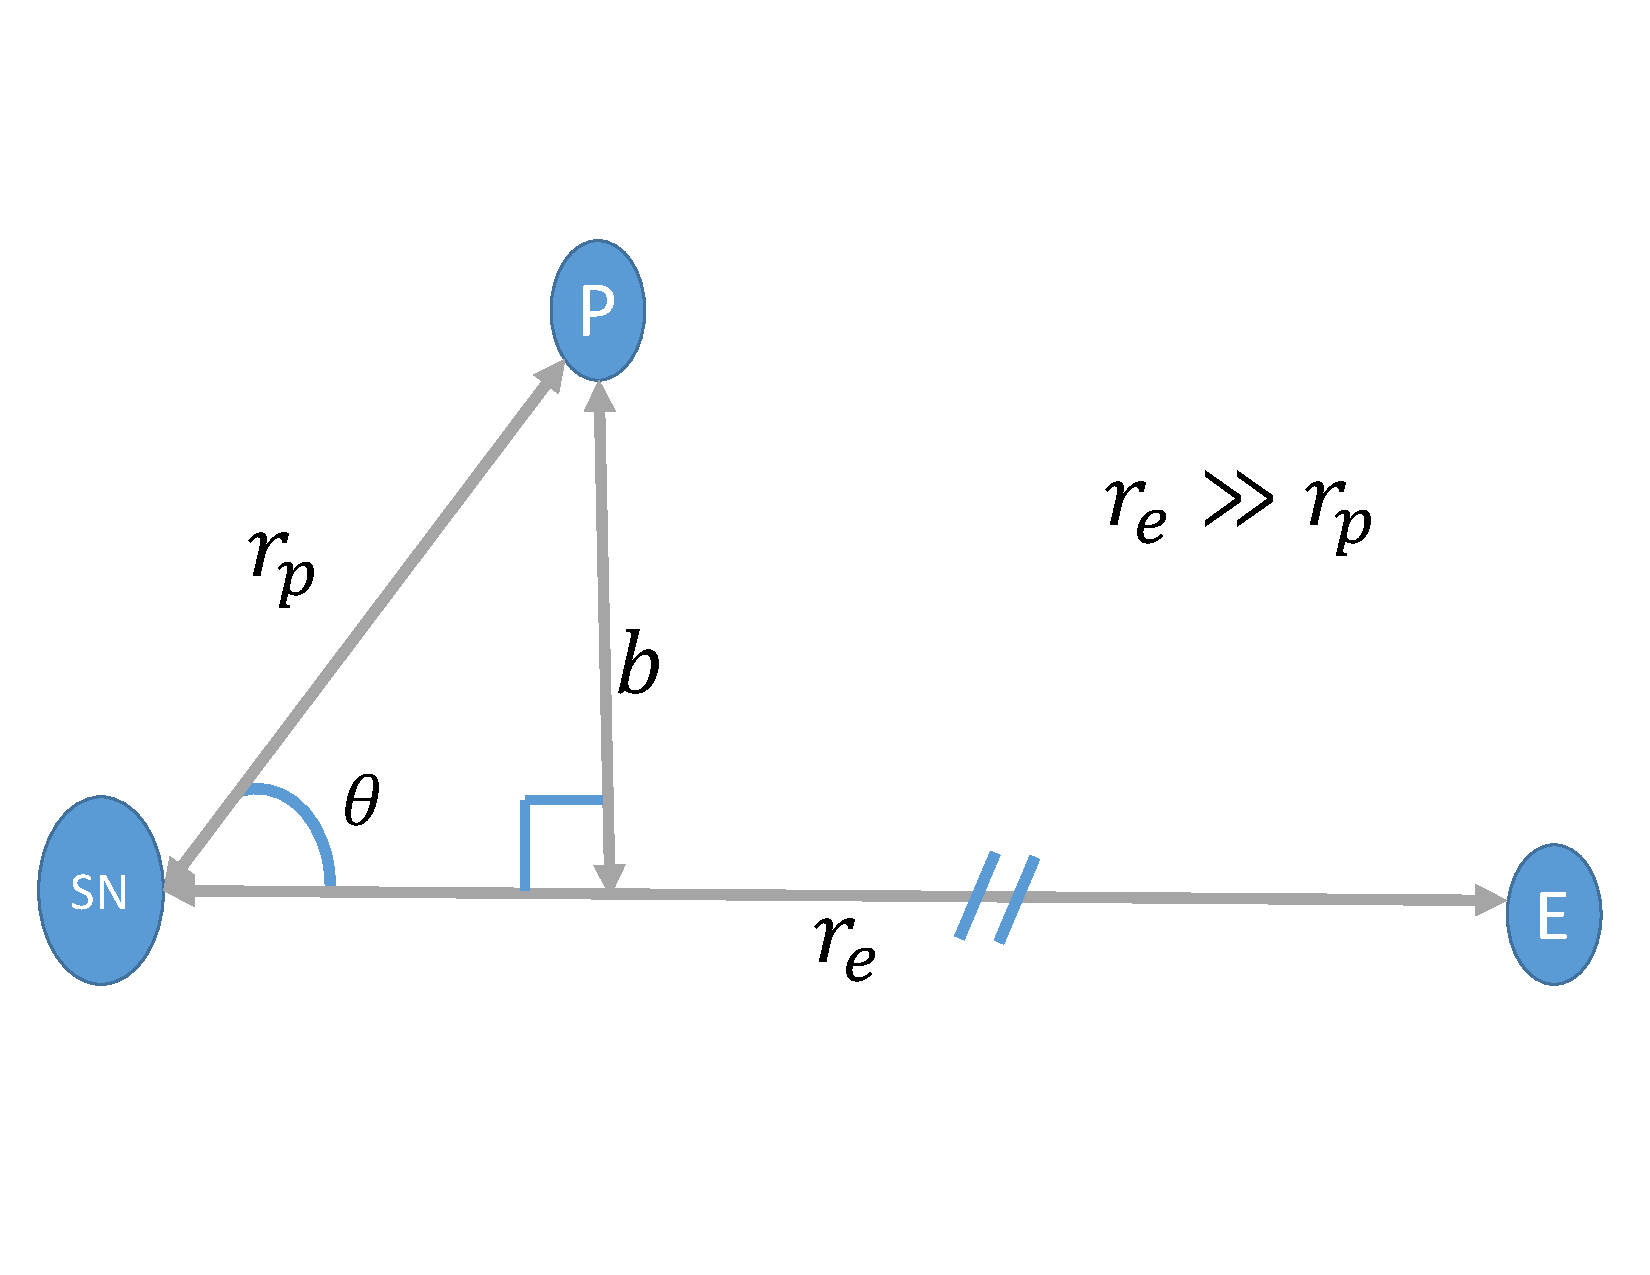
\includegraphics[scale = 0.3]{Image4.pdf}
\vspace{-8 mm}\caption{General geometry of the three objects. Where $b$ is the impact parameter of the photons from pulsar to earth. } 
\label{fig:3}
\end{center}
\end{figure}

Recall that in the aligned case, there was one special ``time'' (a particular photon in the train of signals from the pulsar), before which both the earth and the pulsar are outside the neutrino shell, and after which they are both inside it. In the general case, there are two such special ``time''s, and it is easiest to understand from the special case in which $\theta \approx \pi$, as shown in Fig.\ref{fig-opposite}. $t_1$ is when the neutrino shell passes through the earth, which is also when we observe the SN explosion.  $t_2$ is when the neutrino hits the pulsar, or from the earth's perspective, when we see the first photon from the pulsar after it is hit by the neutrino shell.

\begin{figure}[tb]
\begin{center}
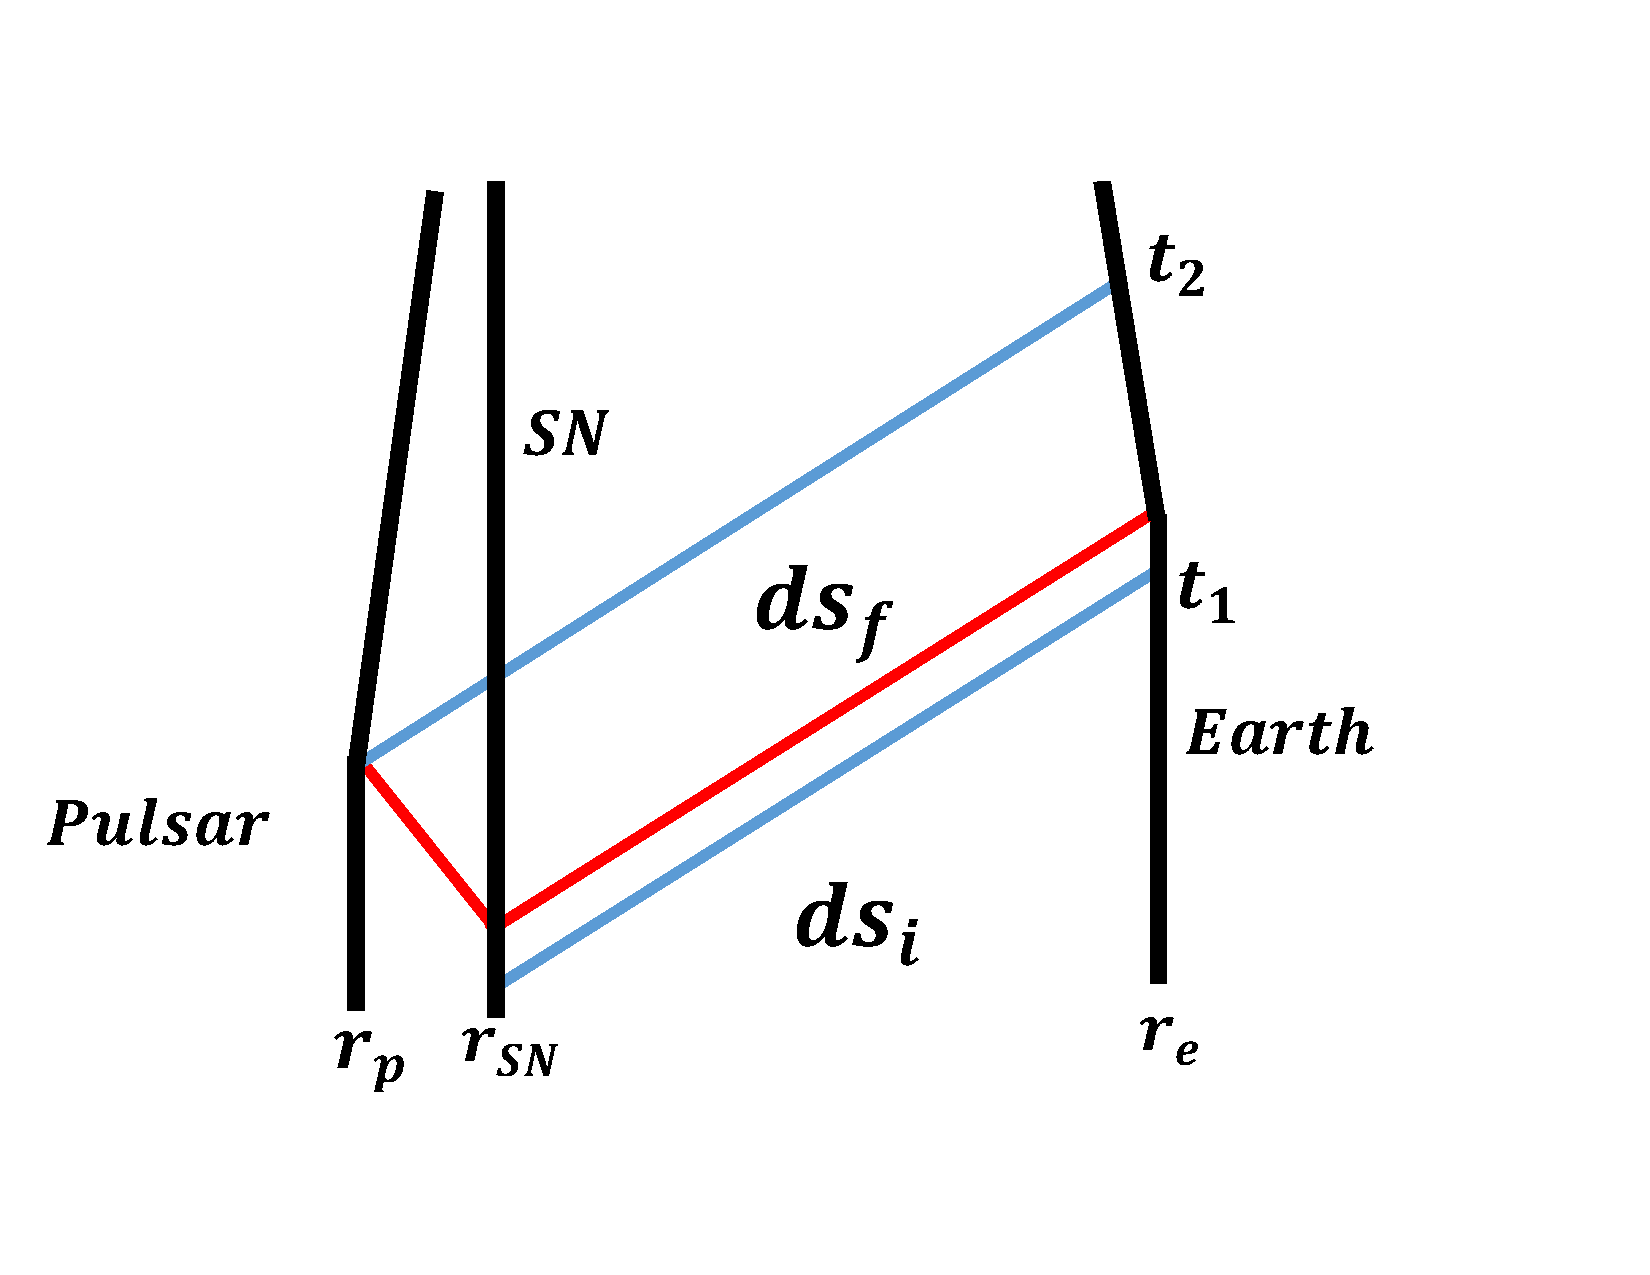
\includegraphics[scale = 0.3]{Image5.pdf}
\caption{Spacetime diagram showing the pulsar at $\theta \approx \pi$ with the same color-code as Fig.\ref{fig:1}. The two photons are right before the first change and right after the second change of $\dot{w_e}$.}
\label{fig-opposite}
\end{center}
\end{figure}

At $t_2$, the sudden change obviously comes from the fact discussed in Sec.\ref{sec-acceleration}: the pulsar is suddenly feeling a different acceleration. The change at $t_1$ has a different reason, since the acceleration change of the earth is tiny when $r_e\gg r_p$. The relevant change is the fact that right before $t_1$, the photon traveling from the pulsar to the earth in the ``initial'' spacetime, but right after $t_1$, it (mostly) travels in the ``final'' spacetime. In fact, between $t_1$ and $t_2$, every photon from the pulsar has to cross the neutrino shell somewhere before reaching the earth. Such process contributes to an extra term to $\dot{w_e}/w_e$. Since the change at $t_2$ is obviously the $\cos\theta$ projection of Eq.~(\ref{eq-AccChange}), we are at the following situation:
\begin{center}
\begin{tabular}{| c | c | c | c |} 
\hline
       & $t<t_1$ & $t_1<t<t_2$ & $t_2<t$ \\ 
       \hline 
$\dot{w_e}/w_e$ &  $-(M_i/r_p^2)\cos\theta$   & $-(M_i/r_p^2)\cos\theta+$?    
& $-(M_f/r_p^2)\cos\theta$   \\ 
\hline 
\end{tabular}
\end{center}
We will proceed to calculate the unknown contribution in the middle stage.

\subsection{Effective acceleration}

Keeping track of how exactly every photon crosses the neutrino shell is a cumbersome task for $\theta\neq 0$ or $\pi$. That would give us the effective acceleration at every instance between $t_1$ and $t_2$, which is too much information to ask for. We always need time for the change in $w_e$ to build up in order to observe it, and we should count ourselves lucky if we can see an average effect in the entire duration,
\begin{equation}
\Delta t = t_2- t_1 = r_p(1-\cos\theta)~.
\end{equation}
Thus we will simply calculate this ``average'' extra contribution to $\dot{w_e}/w_e$, which is much easier.

Right before $t_1$, we can find a photon that travels from the pulsar to the earth totally in the ``initial" geometry. Without loss of generality, we let the pulsar be at rest. Its 4-vector is then given by the first expression in Eq.~(\ref{eq-PulsarRest}). As shown in Fig.\ref{fig:3}, a photon aiming toward the earth must have $b = r_p\sin\theta$. We can then solve for $(w_e)_{t_1} \approx (w_\infty)_{t_1}$ by
\begin{eqnarray}
w_p = -(p_\mu k^\mu)_{\rm i} &=& 
(w_\infty)_{t_1} \left(1-\frac{2M_i}{r_p}\right)^{-1/2}~, \nonumber \\
(w_e)_{t_1} &\approx& w_p \left(1-\frac{M_i}{r_p}\right)~.
\end{eqnarray}
Right after $t_2$, a photon goes from the pulsar to the earth entirely in the ``final" geometry, and $p_\mu$ is given by the second expression of Eq.~(\ref{eq-PulsarRest}). We can similarly solve for $(w_e)_{t_1}\approx (w_\infty)_{t_2}$. 
\begin{eqnarray}
%w_p = -(p_\mu k^\mu)_f 
%&=& (w_\infty)_{t_2} \left[ \left(1-\frac{2M_f}{r_p}\right)^{-1/2} + \sqrt{1-\frac{b^2}{r_p^2 }\left(1-\frac{2M_f}{r_p}\right)} v \left(1-\frac{2M_f}{r_p}\right)^{-1}\right] 
%\nonumber \\
(w_e)_{t_2} &\approx& w_p \left(1-\frac{M_f}{r_p} - \cos\theta \frac{\Delta M}{r_p}\right)~.
\end{eqnarray}
Note that this $p_\mu$ only includes the change due to crossing the shell, without the result of actual acceleration from the SN's gravity. Since the later is already taken into account in the chart of Sec.\ref{sec-3d}, we are indeed calculating the extra contribution to
\begin{equation}
\frac{\dot{w_e}}{w_e}\bigg|_{\rm extra \ from \ t_1 \ to \ t_2} = \frac{(w_e)_{t_2}-(w_e)_{t_1}}{\Delta t} = \frac{\Delta M}{r_p^2}~.
\end{equation}
Interestingly, there is no $\theta$ dependence here.

\section{Observational Practicality}
\label{sec-obs}

The observed value of $(\dot{w_e}/w_e)$ cannot be exactly what we calculated, because in practice, there are many other contributions to the acceleration. For example, both the SN and the pulsar may be in the galactic center which has a relative acceleration to our spiral arm. However, if the pulsar is close enough to the SN, then we can be pretty certain that in the time scale comparable to $\Delta t$, the SN is the dominant cause of acceleration change. % Afterall, there are rarely any event more violent than a nearby SN explosion. And if there is, we probably would have noticed.

That means, if we observe three different values of $(\dot{w_e}/w_e)$ in the three stages, we can subtract the value in the first stage and get two independent data corresponding to the effect we calculated.
\begin{center}
\begin{tabular}{| c | c | c |} 
\hline
                & $t_1<t<t_2$ & $t_2<t$ \\ 
       \hline 
$\Delta(\dot{w_e}/w_e)$ & $ \Delta M/r_p^2$ 
& $(\Delta M/r_p^2)\cos\theta$   \\ 
\hline 
\end{tabular}
\end{center}

If the SN is directly visible, then the angular separation to a nearby pulsar, $r_p\sin\theta$, should be measured quite accurately on its own. The depth difference, $r_p\cos\theta$, may have a large error bar; the actual total energy released in neutrino shell is only estimated from theory. The observation of this two-stage acceleration change then allows us to determine those two values, if the pulsar is sensitive enough to detect an acceleration change of order $\Delta M/r_p^2$.

In practice $\dot{w_e}$ is measured by allowing the signal to build up a frequency change, and then to build up again in the phase change. That means within the duration of the middle stage, the arrival time of the pulse changes by 
\begin{equation}
\delta T_{\rm arrival} \sim \Delta\left(\frac{\dot{w_e}}{w_e}\right)(\Delta t)^2
\sim \Delta M~.
\end{equation}
Interestingly, the $1/r_p^2$ in gravitational force exactly cancels with the accumulation time $(\Delta t)^2$. That means independent of $r_p$, a pulsar can detect this change as long as the timing accuracy is better than the light-crossing time of the effective Schwarzschild radius of the neutrino shell\footnote{In practice, we still want the pulsar to be somewhere close to the SN. Without that condition, we cannot be certain that there are no other comparable changes to acceleration during $\Delta t$.}. We can estimate $\Delta M\sim$ a fraction of solar mass $\sim10^{-6}$ seconds. $\delta T_{\rm arrival}$ for a stable, millisecond pulsar is already better \cite{PulsarTiming}\footnote{Our conservative estimation assumes only two measurements: in the beginning and the end of the duration $\Delta t$. In practice, one has $N$ measurements during the process, which increases the accuracy by another factor of $\sqrt{N}$.}.

With the forecast of thousands of millisecond pulsars to be found by the Square Kilometer Array \cite{SKA}, a new SN effectively sits within a timing-grid. At the instant the SN is detected at earth, even if only from direct neutrino detection, we know that all pulsar timing periodic derivatives change, and by different amounts depending on their distances. The closest or the best timed pulsars may detect such effect within a decade or two, and others gradually follow. Such a joint timing can triangulate the location of the SN and prepare us to detect the second acceleration change. Given a few SN per century\cite{SNrate06}, an actual detection is in the forewseeable future.

% The effect receives equal logarthmic contributions in detectability as a distance of the pulsar from the SN: in a disk population, the number of pulsars increases as the square of the distance from the SN, the effect decreases as the distance, and the sensitivity increases with the square root of the number of pulsars.  Pulsars near the line of sight will increasingly show the second acceleration change, the soonest typically after a year, for the pulsar one galactic scale length from the SN along our line of sight.  THe timing impact will be weak due to its distance from the SN, and waiting for a decade increases both the acceleration sensitivity due to the longer time baseline, and increases the likelihood of finding a pulsar closer to the SNe. 

\acknowledgments

We thank xxx useful discussions. We are supported in part by xxx fundings.

\appendix

%\bibliographystyle{utcaps}
\bibliography{all_active}


\end{document}

